\section{Visualization Result and Conclusion}
Our visualization tool allows users to see the relationship between HDI and its components. As we can see from Figure~\ref{fig:parallelplot}, almost all the countries with high HDI have relatively high values of the four components (LEB, EYS, MYS, GNI). In additions, the bivariate map (Figure~\ref{fig:bivariate}) shows an interesting finding: most of the countries have close values of GNI per capita, regardless of how many expected years of schooling people have. Figure~\ref{fig:parallelplot} shows that all the countries except only one country have GNI per capita under 80000 in 2015. The only one country with the highest GNI per capita is Qatar. Another finding is that the countries located in the lower part of the earth tend to have low expected years of schooling as shown in our tool by showing only countries (on the world map) with values of the low expected years of schooling. The world map (Figure~\ref{fig:hdi}) also leads to the conclusion that Africa is the continent that has the relatively low human development as most of the countries in Africa have low HDI. However, by using the year slider controller, we can see that the majority of the countries have been developed in the past several years, because their HDI values are increasing as the years go by. 

\begin{figure}[t]
    \centering
    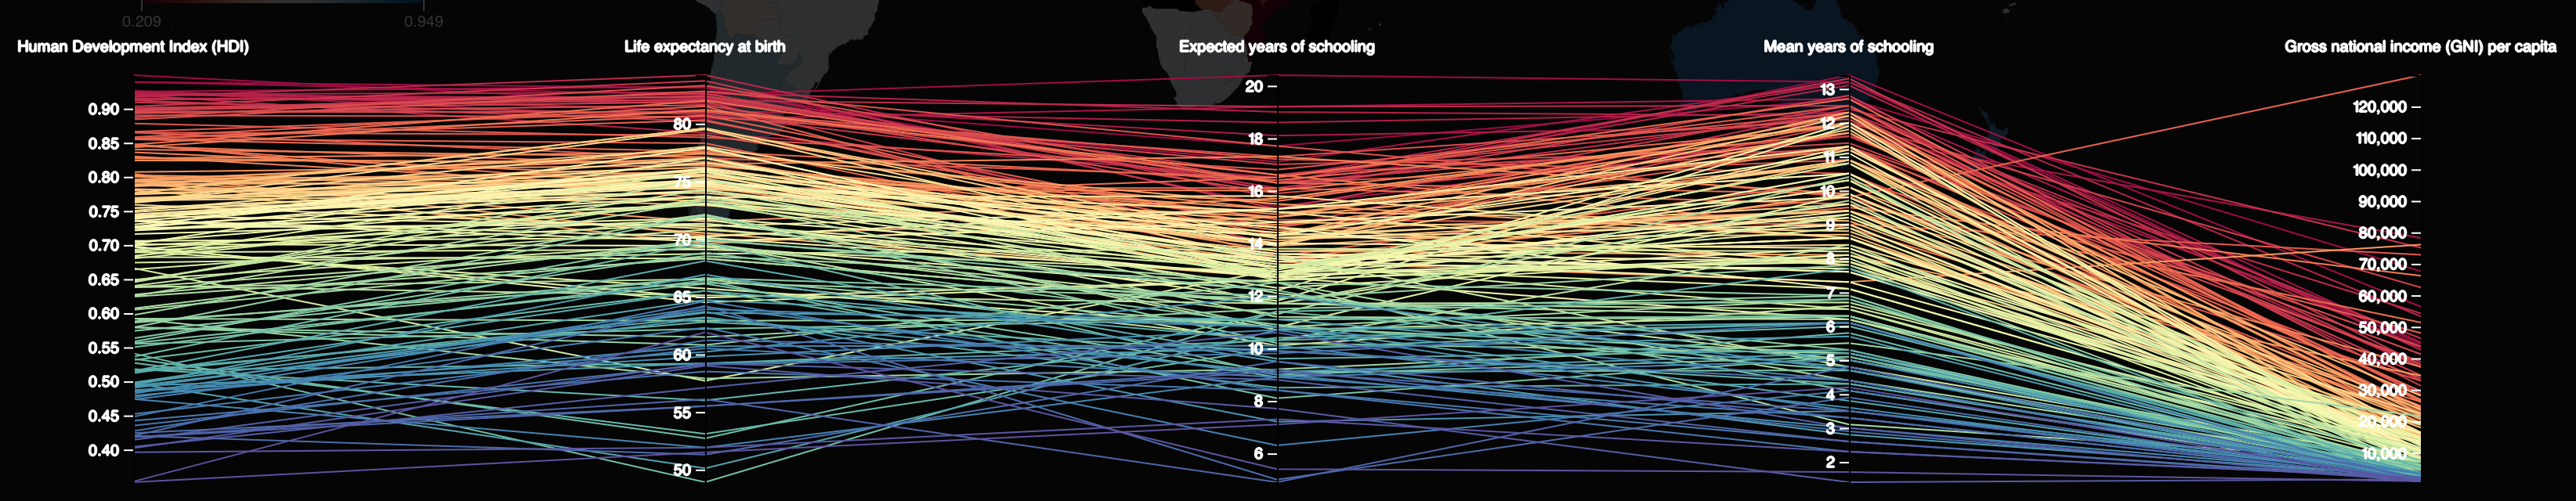
\includegraphics[width=0.4\textwidth]{parallelplot}
    \caption{Parallel Coordinate Plot showing the HDI and its components of each country in 2015}
    \label{fig:parallelplot}
\end{figure}
